%%%%%%%%%%%%%%%%%%%%%%%%%%%%%%%%%%%%%%%%%
% UHCL Computer Architecture Final Project
% Laboratory Report
%
% Original author:
% Mike Moore
%
%%%%%%%%%%%%%%%%%%%%%%%%%%%%%%%%%%%%%%%%%

%----------------------------------------------------------------------------------------
%  PACKAGES AND DOCUMENT CONFIGURATIONS
%----------------------------------------------------------------------------------------

\documentclass{article}

\usepackage{graphicx} % Required for the inclusion of images
\usepackage{listings}
\usepackage{courier}
\usepackage{color}
\usepackage{caption}
\usepackage{graphics}

% Settings for the VHDL Code Listings.

\definecolor{javared}{rgb}{0.6,0,0} % for strings
\definecolor{javagreen}{rgb}{0.25,0.5,0.35} % comments
\definecolor{javapurple}{rgb}{0.5,0,0.35} % keywords
\definecolor{javadocblue}{rgb}{0.25,0.35,0.75} % javadoc
 
\lstset{
      basicstyle=\footnotesize\ttfamily, % Standardschrift
      %numbers=left,               % Ort der Zeilennummern
      numberstyle=\tiny,          % Stil der Zeilennummern
      %stepnumber=2,               % Abstand zwischen den Zeilennummern
      numbersep=5pt,              % Abstand der Nummern zum Text
      tabsize=2,                  % Groesse von Tabs
      extendedchars=true,         %
      breaklines=true,            % Zeilen werden Umgebrochen
      keywordstyle=\color{red},
      frame=b,         
%        keywordstyle=[1]\textbf,    % Stil der Keywords
%        keywordstyle=[2]\textbf,    %
%        keywordstyle=[3]\textbf,    %
%        keywordstyle=[4]\textbf,   \sqrt{\sqrt{}} %
      stringstyle=\color{white}\ttfamily, % Farbe der String
      showspaces=false,           % Leerzeichen anzeigen ?
      showtabs=false,             % Tabs anzeigen ?
      xleftmargin=17pt,
      framexleftmargin=17pt,
      framexrightmargin=5pt,
      framexbottommargin=4pt,
      %backgroundcolor=\color{lightgray},
      showstringspaces=false      % Leerzeichen in Strings anzeigen ?        
 }
 \lstloadlanguages{% Check Dokumentation for further languages ...
         VHDL
 }
\lstset{language=VHDL,
basicstyle=\ttfamily,
keywordstyle=\color{javapurple}\bfseries,
stringstyle=\color{javared},
commentstyle=\color{javagreen},
morecomment=[s][\color{javadocblue}]{/**}{*/},
stepnumber=1,
numbersep=3pt,
tabsize=2,
showspaces=false,
showstringspaces=false}

% Captions for VHDL Code Snippets
\DeclareCaptionFont{blue}{\color{blue}} 

% Captions for VHDL Code Snippets
%\DeclareCaptionFont{blue}{\color{blue}} 

%\captionsetup[lstlisting]{singlelinecheck=false, labelfont={blue}, textfont={blue}}
\usepackage{caption}
\DeclareCaptionFont{white}{\color{white}}
\DeclareCaptionFormat{listing}{\colorbox[cmyk]{0.43, 0.35, 0.35,0.01}{\parbox{\textwidth}{\hspace{15pt}#1#2#3}}}
\captionsetup[lstlisting]{format=listing,labelfont=white,textfont=white, singlelinecheck=false, margin=0pt, font={bf,footnotesize}}


\setlength\parindent{0pt} % Removes all indentation from paragraphs

\renewcommand{\labelenumi}{\alph{enumi}.} % Make numbering in the enumerate environment by letter rather than number (e.g. section 6)

%----------------------------------------------------------------------------------------
%  DOCUMENT INFORMATION
%----------------------------------------------------------------------------------------

\title{Design of a 4-bit ALU \\ Using VHDL \\ CENG 3511} % Title

\author{Mike \textsc{Moore}} % Author name

\date{\today} % Date for the report

\begin{document}

\maketitle % Insert the title, author and date

\begin{center}
\begin{tabular}{l r}
Date Performed: & November 17 2013 \\ % Date the experiment was performed
Instructor: & Dr. George Collins % Instructor/supervisor
\end{tabular}
\end{center}




% If you wish to include an abstract, uncomment the lines below
\begin{abstract}
The objective of the project is to implement a four-bit arithmetic logic unit for a
processor. The basic requirements include the following fundamental operations:
addition, increment, decrement, transfer, and the basic logical operations
(AND, OR, NOT, XOR). A behavioral approach is taken to implement this ALU. The VHDL
defines inputs for two four bit registers, a four bit op-code field, and a single 
carry in bit. The outputs are the four bit data out, and the single carry out bit. 
From a block diagram of the ALU design, a VHDL module is developed to satisfy the
design requirements. This VHDL module is then put under test and the results are 
examined.
\end{abstract}

\newpage

\tableofcontents

\newpage

%----------------------------------------------------------------------------------------
%  SECTION 1
%----------------------------------------------------------------------------------------

%%%%%%%%%%%%%%%%%%%%%%%%%%%%%%%%%%%%%%%%%%%%%%%%%%%%%%%%%%%%
\section{Introduction}

An Arithmetic Logic Unit (ALU) is a fundamental component within the central processing
unit (CPU). It is responsible for both the arithmetic and logical operations of the CPU,
and as such, it is responsible for a large part of the CPU work load. Modern ALU designs
can be quite complex, and often they are not actually a single unit within the CPU. For 
simplicity, this report focuses on a simplified four bit ALU design.

%----------------------------------------------------------------------------------------
%  SECTION 1
%----------------------------------------------------------------------------------------

%%%%%%%%%%%%%%%%%%%%%%%%%%%%%%%%%%%%%%%%%%%%%%%%%%%%%%%%%%%%
\section{Preliminary Design}
The design begins with an evaluation of a list of design requirements. The requirements include a table
of operations that the ALU must implement. From this table, a set of validation criteria
can be derived. This validation criteria directly leads to a set of tests that can be used 
to validate that the ALU performs all of the desired functions.


\subsection{ALU Requirements}
The ALU was designed to meet the following list of requirements:

\begin{itemize}
   \item The unit has two 4-bit inputs, register A and register B. 
   \item The unit must be able to add, increment, decrement, transfer and also perform basic logic operations AND, OR, NOT, XOR. 
   \item The unit will have 4-bit select line called Operation Select, which would direct the unit as to which operation to perform. 
   \item In addition the unit must also be able to do shift operations (right shift, left shift etc). 
   \item The unit has a Carry-in and also has Carry-out. 
\end{itemize}

We see from the above requirements list that we will need to design an ALU that has a total of thirteen
input bits. Eight will be used for the two four bit operand registers, and another four will be used for
the op-code. Finally, a single carry in bit is also required. The outputs are a little bit simpler. We will only need four bits for the data out, and a single bit for the carry out.

\newpage

\subsection{ALU Block Diagram}
With this understanding of our requirements, the next step is to depict the ALU in a functional block diagram form. This will later allow for us to more easily translate the preliminary design to a VHDL module. The block diagram description of our ALU is provided below. Note how the inputs and outputs directly map to statements in the list of requirements.
\begin{figure}[ht!]
\centering
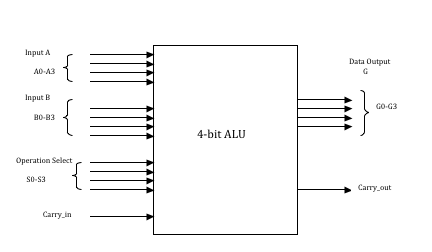
\includegraphics[width=100mm, height=50mm]{images/BlockDiagramALU.png}
\caption{Four Bit ALU Block Diagram}
\label{overflow}
\end{figure}

\subsection{ALU Operations}
The required operations for the ALU are listed below.
\begin{figure}[ht!]
\centering
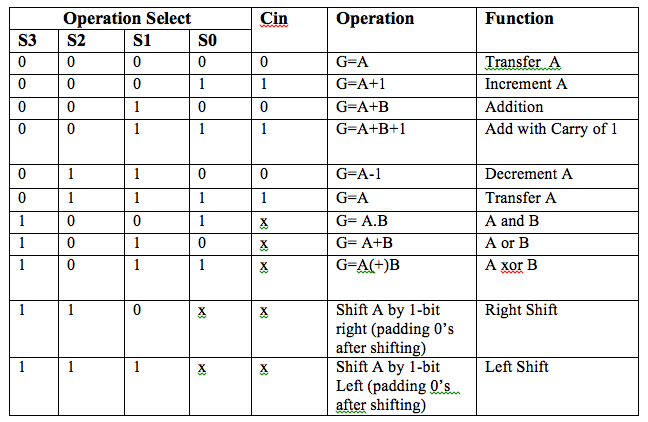
\includegraphics[width=100mm, height=50mm]{images/ALUOps.png}
\caption{Four Bit ALU Required Operations} 
\label{overflow}
\end{figure}



%----------------------------------------------------------------------------------------
%  SECTION 3
%----------------------------------------------------------------------------------------

%%%%%%%%%%%%%%%%%%%%%%%%%%%%%%%%%%%%%%%%%%%%%%%%%%%%%%%%%%%%
\section{The ALU VHDL Module}

The next step in the ALU design process was to actually write out the
VHDL to perform the desired functions. A behavioral model is used to implement
the ALU. This makes the code more readable at the expense of obfuscating the underlying
hardware implementation. A structural model would be more revealing in that case, but for
the sake of code readability and ease of implementation, a behavioral model was decided upon
for this design.

\subsection{ALU VHDL Code}
The most noteworthy aspect of the VHDL module that was developed is the switch case 
statement that implements the ALU operations table in section 2.3. This switch case evaluates
the four input op-code bits and performs the desired operation on the two register inputs. 
Another thing to take notice of is the use of standard logical vectors for the four bit
operands and op-code. The data out also utilizes a standard logical vector. This simplifies the
code and makes it much more readable. However, it does require a careful interpretation of the
test bench waveform displayed in the results section.

\lstinputlisting[label=aluCode,caption=Four Bit ALU VHDL Code]{FourBitALU/FourBitALU.vhd}

\subsection{ALU VHDL Test Code}
With the primary ALU VHDL module developed, we turn to creating a test to verify the ALU 
implementation against the requirements listed in section 2. This test will be implemented
as a VHDL module so that we can use the Xilinx ISE Design Suite Simulation Test Bench to
run a simulated test of our ALU. The test will perform one or two checks for each operation
in the ALU operations table defined in section 2.3. Test inputs and expected outputs are 
clearly listed in the comments of the test code.

\lstinputlisting[label=aluCode,caption=Four Bit ALU Test Code]{FourBitALU/TestFourBitALU.vhd}
\newpage

%----------------------------------------------------------------------------------------
%  SECTION 4
%----------------------------------------------------------------------------------------

\section{Results}
The Xilinx ISE Design Suite Simulation Test Bench was used to run the tests against the
four bit ALU VHDL module. The results of the test are depicted below as a time history
of the input and output waveform.

\label{definitions}

\begin{figure}[ht!]
\centering
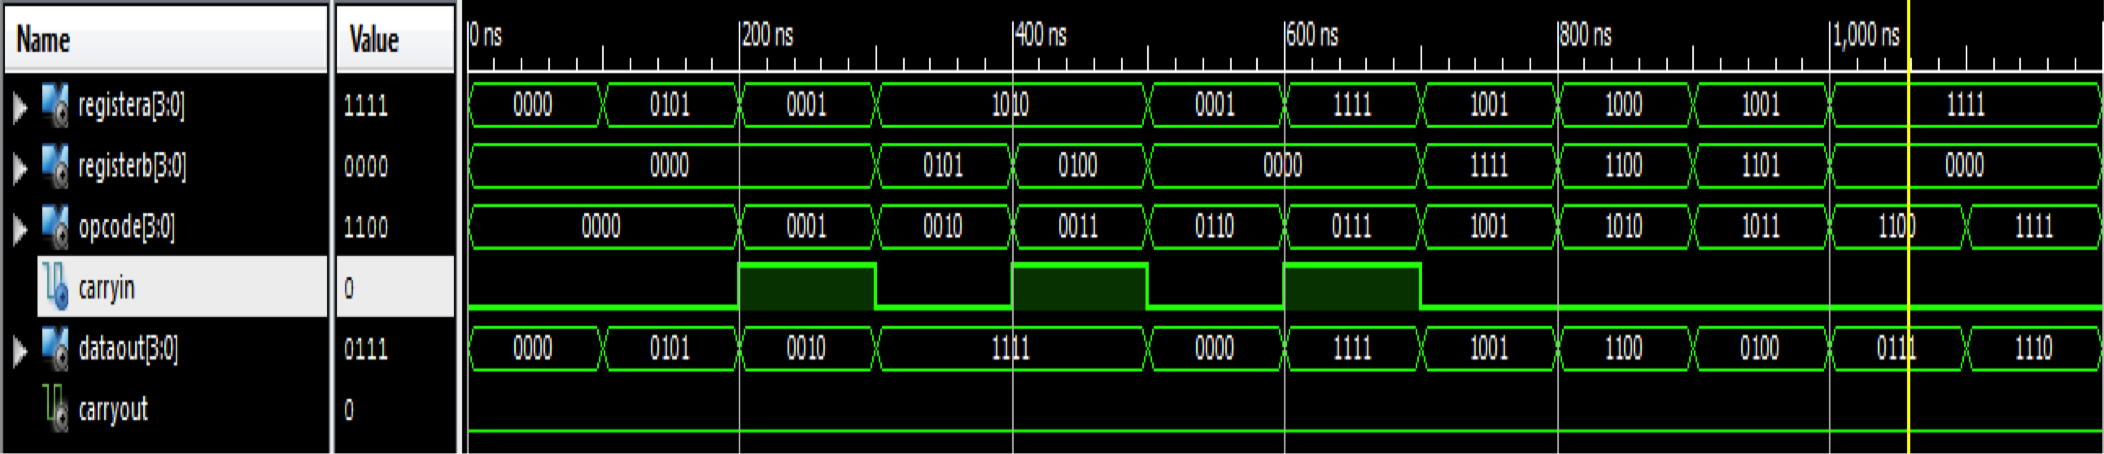
\includegraphics[width=122mm, height=50mm]{images/ALUResults.png}
\caption{Four Bit ALU Required Operations} 
\label{overflow}
\end{figure}

\subsection{Verification of Waveform Plot}
As an example, let's use this plot to verify our test of the addition operation of the
ALU. Use the plot above to examine the input/output waveform at time 300ns. We can see
that the desired op-code is 0010. This corresponds to the addition operation in the ALU
operations table in section 2.3. The register inputs can be seen in the plot above.
Register A is 1010, and register B is 0101. The expected sum of these two is 1111 with 
no carry out. If you examine the output waveform, you will see exactly that result. The
remaining operations and their correctness can be evaluated in the same way.

%----------------------------------------------------------------------------------------
%  SECTION 5
%----------------------------------------------------------------------------------------

\section{Conclusions}
The design and implementation of the simplified four bit ALU was carried out utilizing
a logical progression that starts with requirement definition, moves on to preliminary design,
VHDL implementation, and finally verification and validation using simulation. This process
produces a design for a four bit ALU that can be taken to a hardware implementation on a 
CPLD. The verification and validation steps use simulation to bolster confidence that the 
design will work upon implementation on a CPLD. A hardware implementation was not listed in the
project requirements, and as such, it is left as a follow on exercise. The ALU is a conceptually
simple but nevertheless critical component in the CPU, and this exercise provided valuable
insight into the CPU and computer architecture in general.


\end{document}
